\documentclass[11pt]{article}

\usepackage[T1]{fontenc}
\usepackage{lmodern}
\usepackage[margin=1in]{geometry}
\usepackage{amsmath,amssymb}
\usepackage{booktabs}
\usepackage{graphicx}
\usepackage{float}
\usepackage{microtype}
\usepackage{siunitx}
\usepackage{natbib}
\usepackage{hyperref}
\usepackage{xcolor}
\usepackage{enumitem}
\usepackage{array}
\usepackage{longtable}
\usepackage{caption}
\usepackage{subcaption}

\hypersetup{
  colorlinks=true,
  linkcolor=black,
  citecolor=blue!55!black,
  urlcolor=blue!55!black,
  pdftitle={Design and Validation of a Market-Neutral Cross-Sectional Reversal Strategy},
  pdfauthor={Noah Huerta}
}

\graphicspath{{figures/}}
\setlength{\parindent}{0pt}
\setlength{\parskip}{0.55em}
\setlist[itemize]{topsep=0.25em,itemsep=0.2em}
\captionsetup{font=small,labelfont=bf}
\sisetup{detect-all}

\newcommand{\bps}{\,\mathrm{bps}}
\newcommand{\NAV}{\mathrm{NAV}}
\newcommand{\IR}{\mathrm{IR}}
\newcommand{\IC}{\mathrm{IC}}
\newcommand{\BR}{\mathrm{BR}}
\newcommand{\TC}{\mathrm{TC}}

\title{\textbf{Design and Validation of a Market-Neutral Cross-Sectional Reversal Strategy}\\[0.5em]
\large Quantitative Finance Capstone Report}
\author{Noah Huerta}
\date{September 2026}

\begin{document}
\maketitle

\begin{abstract}
This study develops and evaluates a systematic U.S. equity long--short strategy designed to isolate cross-sectional
return predictability while minimizing exposure to the broad market and industry structure. The strategy combines three
forecasting sleeves---volume-shock reversal, overnight reversal, and post-earnings-announcement drift---within a
dollar-, beta-, and sector-neutral portfolio. Signals are winsorized and standardized cross-sectionally, combined into a
single alpha score, translated into risk-scaled positions using a Ledoit--Wolf covariance estimate, and subjected to
position, gross-exposure, and liquidity constraints. Execution occurs at the next market open and includes commissions,
regulatory fees, borrow costs, spread costs, and square-root market impact.

The final strategy is evaluated on 2015--2024 U.S. large-cap data using a 13-fold walk-forward procedure with a
holding-period embargo and explicit accounting for 327 configurations explored during research, or 355 including the
final validation grid. The delivered configuration earns a walk-forward out-of-sample net Sharpe ratio of 0.901 with a
maximum drawdown of 5.10\%. Modeled trading costs total approximately 63.5 basis points of net asset value per year,
and the estimated break-even cost multiplier is 6.44. The principal empirical finding is that diversification across
weakly correlated signals and effective breadth matter more than maximizing standalone signal strength or relaxing
portfolio constraints. The study also documents negative results, implementation
failures, and limitations---especially survivorship bias and calibrated rather than directly observed trading
spreads---to distinguish evidence from backtest optimism.
\end{abstract}

\section{Introduction}

Short-horizon equity reversal is a natural setting for a quantitative capstone because the economic intuition is simple while the implementation is not. A recent price move may partially reverse when it reflects transient liquidity pressure rather than permanent information. At the same time, the apparent edge is small enough that data timing, portfolio constraints, transaction costs, and repeated parameter search can easily dominate the result. The central question of this project is therefore not merely whether a reversal signal can be found, but whether a diversified reversal book remains economically and statistically credible after realistic portfolio construction, trading costs, and out-of-sample validation.

The strategy studied here is explicitly cross-sectional. It does not forecast the sign of the aggregate equity market. On each trading date, securities are ranked relative to one another by a signed forecast score. Names with the highest scores are held long and those with the lowest are held short, with position size increasing in the score's distance from the cross-sectional mean. Conviction is therefore expressed by that distance in either direction: a name scoring near the mean receives little or no weight, while the most heavily shorted names carry as strong a forecast as the largest longs. The delivered portfolio is constructed to be approximately neutral to dollars, market beta, and GICS sectors. This design makes the return stream primarily a test of stock ordering rather than a disguised directional equity position.

The final forecasting model combines three sleeves. The first is a two-day reversal
signal whose magnitude is conditioned on abnormal volume; the second reverses recent
overnight gaps; and the third uses point-in-time earnings surprises that decay over a
60-trading-day horizon. Each rests on a different economic mechanism, and because they
are only weakly correlated with one another, averaging them yields a more reliable forecast than
any one of them alone: combining volume-shock and overnight reversal raises gross
Sharpe from 0.68 to 0.91, while adding the earnings sleeve improves the out-of-sample
result further.

The report is organized as follows. Section~\ref{sec:data} describes the data and universe. Sections~\ref{sec:signals}--\ref{sec:execution} describe signal construction, portfolio formation, and execution costs. Section~\ref{sec:validation} presents the validation design. Section~\ref{sec:results} reports performance and capacity. Section~\ref{sec:diagnostics} interprets the result through information coefficient, effective breadth, and transfer coefficient. Sections~\ref{sec:robustness} and \ref{sec:limitations} discuss robustness, rejected extensions, and limitations, followed by reproducibility and conclusions.

\section{Data and Tradable Universe}
\label{sec:data}

The research sample spans 2 January 2015 through 31 December 2024, covering 2,516 trading days. Daily market data are collected for 496 tickers, while the fundamental database contains 138,678 SEC XBRL facts across 503 tickers. The tradable universe is refreshed monthly and consists of the 100 most liquid U.S. large-cap common stocks drawn from current S\&P 500 membership. Liquidity is measured using trailing 63-day average dollar volume (ADV), lagged by one trading day. Securities must trade above \$5 and have at least 252 observations of price history, hence the seven ticker difference between the market data and fundamental coverage. Because of this history requirement, the first year of the sample is a warm-up: the book takes its first positions on 14 January 2016, after 260 trading days with no holdings. All data was obtained through the yahoo finance python package and Interactive Brokers API for market data and the SEC XBRL database for fundamental data.

Point-in-time treatment of accounting data is especially important. A fiscal-period end date is not the date at which the information was publicly tradable. The implementation therefore uses the SEC filing date as the visibility date. This avoids the error of assigning December-quarter information to December when the corresponding 10-Q or 10-K may not be filed until weeks later. It also handles restatements naturally because a later filing is can't to overwrite what the market knew historically.

One material data limitation remains: historical index membership is not point-in-time. The S\&P 500 constituent list is seeded from a current snapshot, and delisted firms are absent from yfinance. This introduces a survivor bias and is discussed explicitly in Section~\ref{sec:limitations}.

\section{Signal Construction}
\label{sec:signals}

The strategy combines three economically distinct forecasting sleeves. Short-horizon reversal has long been documented as a form of return predictability \citep{lehmann1990,lomackinlay1990,jegadeesh1990}, while post-earnings-announcement drift (PEAD) shows a delayed implementation of earnings information \citep{bernard1989,bernard1990}. The project does not assume that these effects are naively tradable, each candidate signal must survive the same standardization, execution, and validation framework.

\subsection{Volume-shock reversal}

The first sleeve reverses a two-day stock return, with greater weight placed on moves accompanied by unusually high volume. The economic interpretation is that unusually large price movement combined with a volume shock is more likely to contain temporary liquidity demand, following the volume--autocorrelation relationship documented by \citet{cgw1993}: a move on heavy volume more often reflects a liquidity-motivated order and reverts, whereas the same move on light volume more often reflects information and is therefore more stable. The baseline for ``normal'' volume is 63 trading days. For each sleeve and day, the raw signal is winsorized at three median absolute deviations about the
cross-sectional median before standardization.
\subsection{Overnight reversal}

The second sleeve sums recent overnight price gaps over a five-day lookback and takes the opposite side. The overnight session is relatively thin and order-driven, so some price pressure may reverse during regular trading; \citet{lps2019} document systematically opposite predictability in the overnight and intraday components of returns. Importantly, the overnight signal is not simply a repackaging of the total-return reversal sleeve: its measured correlation with the volume-shock reversal signal is only 0.30.

\subsection{Earnings surprise}

The third sleeve is event-driven. Each newly filed quarterly net income is compared with the value filed four quarterly filings earlier (a seasonal random walk, approximating the same fiscal quarter one year before) and scaled by the standard deviation of the firm's eight most recent such changes, including the current one. The resulting score decays linearly to zero over 60 trading days. This construction seeks a PEAD-type effect while retaining exact filing-date timing. The event clock is crucial: unlike slowly changing valuation ratios, the earnings score arrives discretely and then decays, producing greater effective breadth.

\subsection{Cross-sectional normalization and blending}

For each sleeve $s$ and day $t$, the raw cross-section is winsorized and standardized. If $x_{i,t}^{(s)}$ denotes the clipped raw signal for security $i$, the standardized score is
\begin{equation}
 z_{i,t}^{(s)} = \frac{x_{i,t}^{(s)}-\bar{x}_{t}^{(s)}}{\sigma_t^{(s)}}.
\end{equation}
Standardizing before combination prevents a signal with mechanically larger units from dominating the blend. The final score is
\begin{equation}
 \alpha_{i,t}=0.45z_{i,t}^{\mathrm{VR}}+0.45z_{i,t}^{\mathrm{ON}}+0.10z_{i,t}^{\mathrm{PEAD}},
\end{equation}
where VR denotes volume-shock reversal, ON overnight reversal, and PEAD the earnings-surprise sleeve. The weights are renormalized over the sleeves available for each name, and the blended score is standardized cross-sectionally once more before portfolio construction. The 10\% earnings weight is the best cell of a coarse sweep, with performance falling on both sides of it, so it is a tuned choice rather than a neutral default; for that reason the weight is re-selected inside each walk-forward training window rather than fixed with full-sample hindsight.

Throughout this report, two sleeves are described as weakly correlated on the basis of their average cross-sectional score correlation. On each day $t$, the standardized scores of sleeves $a$ and $b$ form two vectors over the $N_t$ names in the tradable universe $\mathcal{U}_t$, and the correlation is taken \emph{across those names}:
\begin{equation}
 \rho_{ab,t}=\frac{\sum_{i\in\mathcal{U}_t} z_{i,t}^{(a)} z_{i,t}^{(b)}}
 {\sqrt{\sum_{i\in\mathcal{U}_t}\bigl(z_{i,t}^{(a)}\bigr)^{2}}\;
  \sqrt{\sum_{i\in\mathcal{U}_t}\bigl(z_{i,t}^{(b)}\bigr)^{2}}},
 \qquad
 \bar{\rho}_{ab}=\frac{1}{T}\sum_{t=1}^{T}\rho_{ab,t}.
\label{eq:sleevecorr}
\end{equation}
The cross-sectional means are zero by construction after standardization, so no centering term appears. Each day therefore yields a single correlation over the cross-section, and the reported figure is the time-series mean of that daily series. The measure is taken across names within a day rather than along the time axis because the portfolio is determined by the within-day ranking: the relevant question is whether two sleeves want to hold the same securities on the same day. It is consequently distinct both from the average per-name time-series correlation of the two scores and from the correlation of the sleeves' standalone return streams.

Equation~\eqref{eq:blendic} below supplies the scale against which $\bar{\rho}_{ab}$ should be read. For two sleeves the composite skill multiplier is $\sqrt{2/(1+\bar{\rho})}$, which equals 1.41 at $\bar{\rho}=0$ and falls to 1.01 at $\bar{\rho}=0.95$. The redundant within-family pairs in Figure~\ref{fig:corr} sit at 0.94--0.97 and therefore retain under 4\% of the diversification benefit available at zero correlation, whereas the selected pair at 0.30 retains 58\%. ``Weakly correlated'' in this report means a correlation low enough to retain a material share of that multiplier.

\begin{figure}[H]
\centering
\IfFileExists{sleeve_correlations.png}{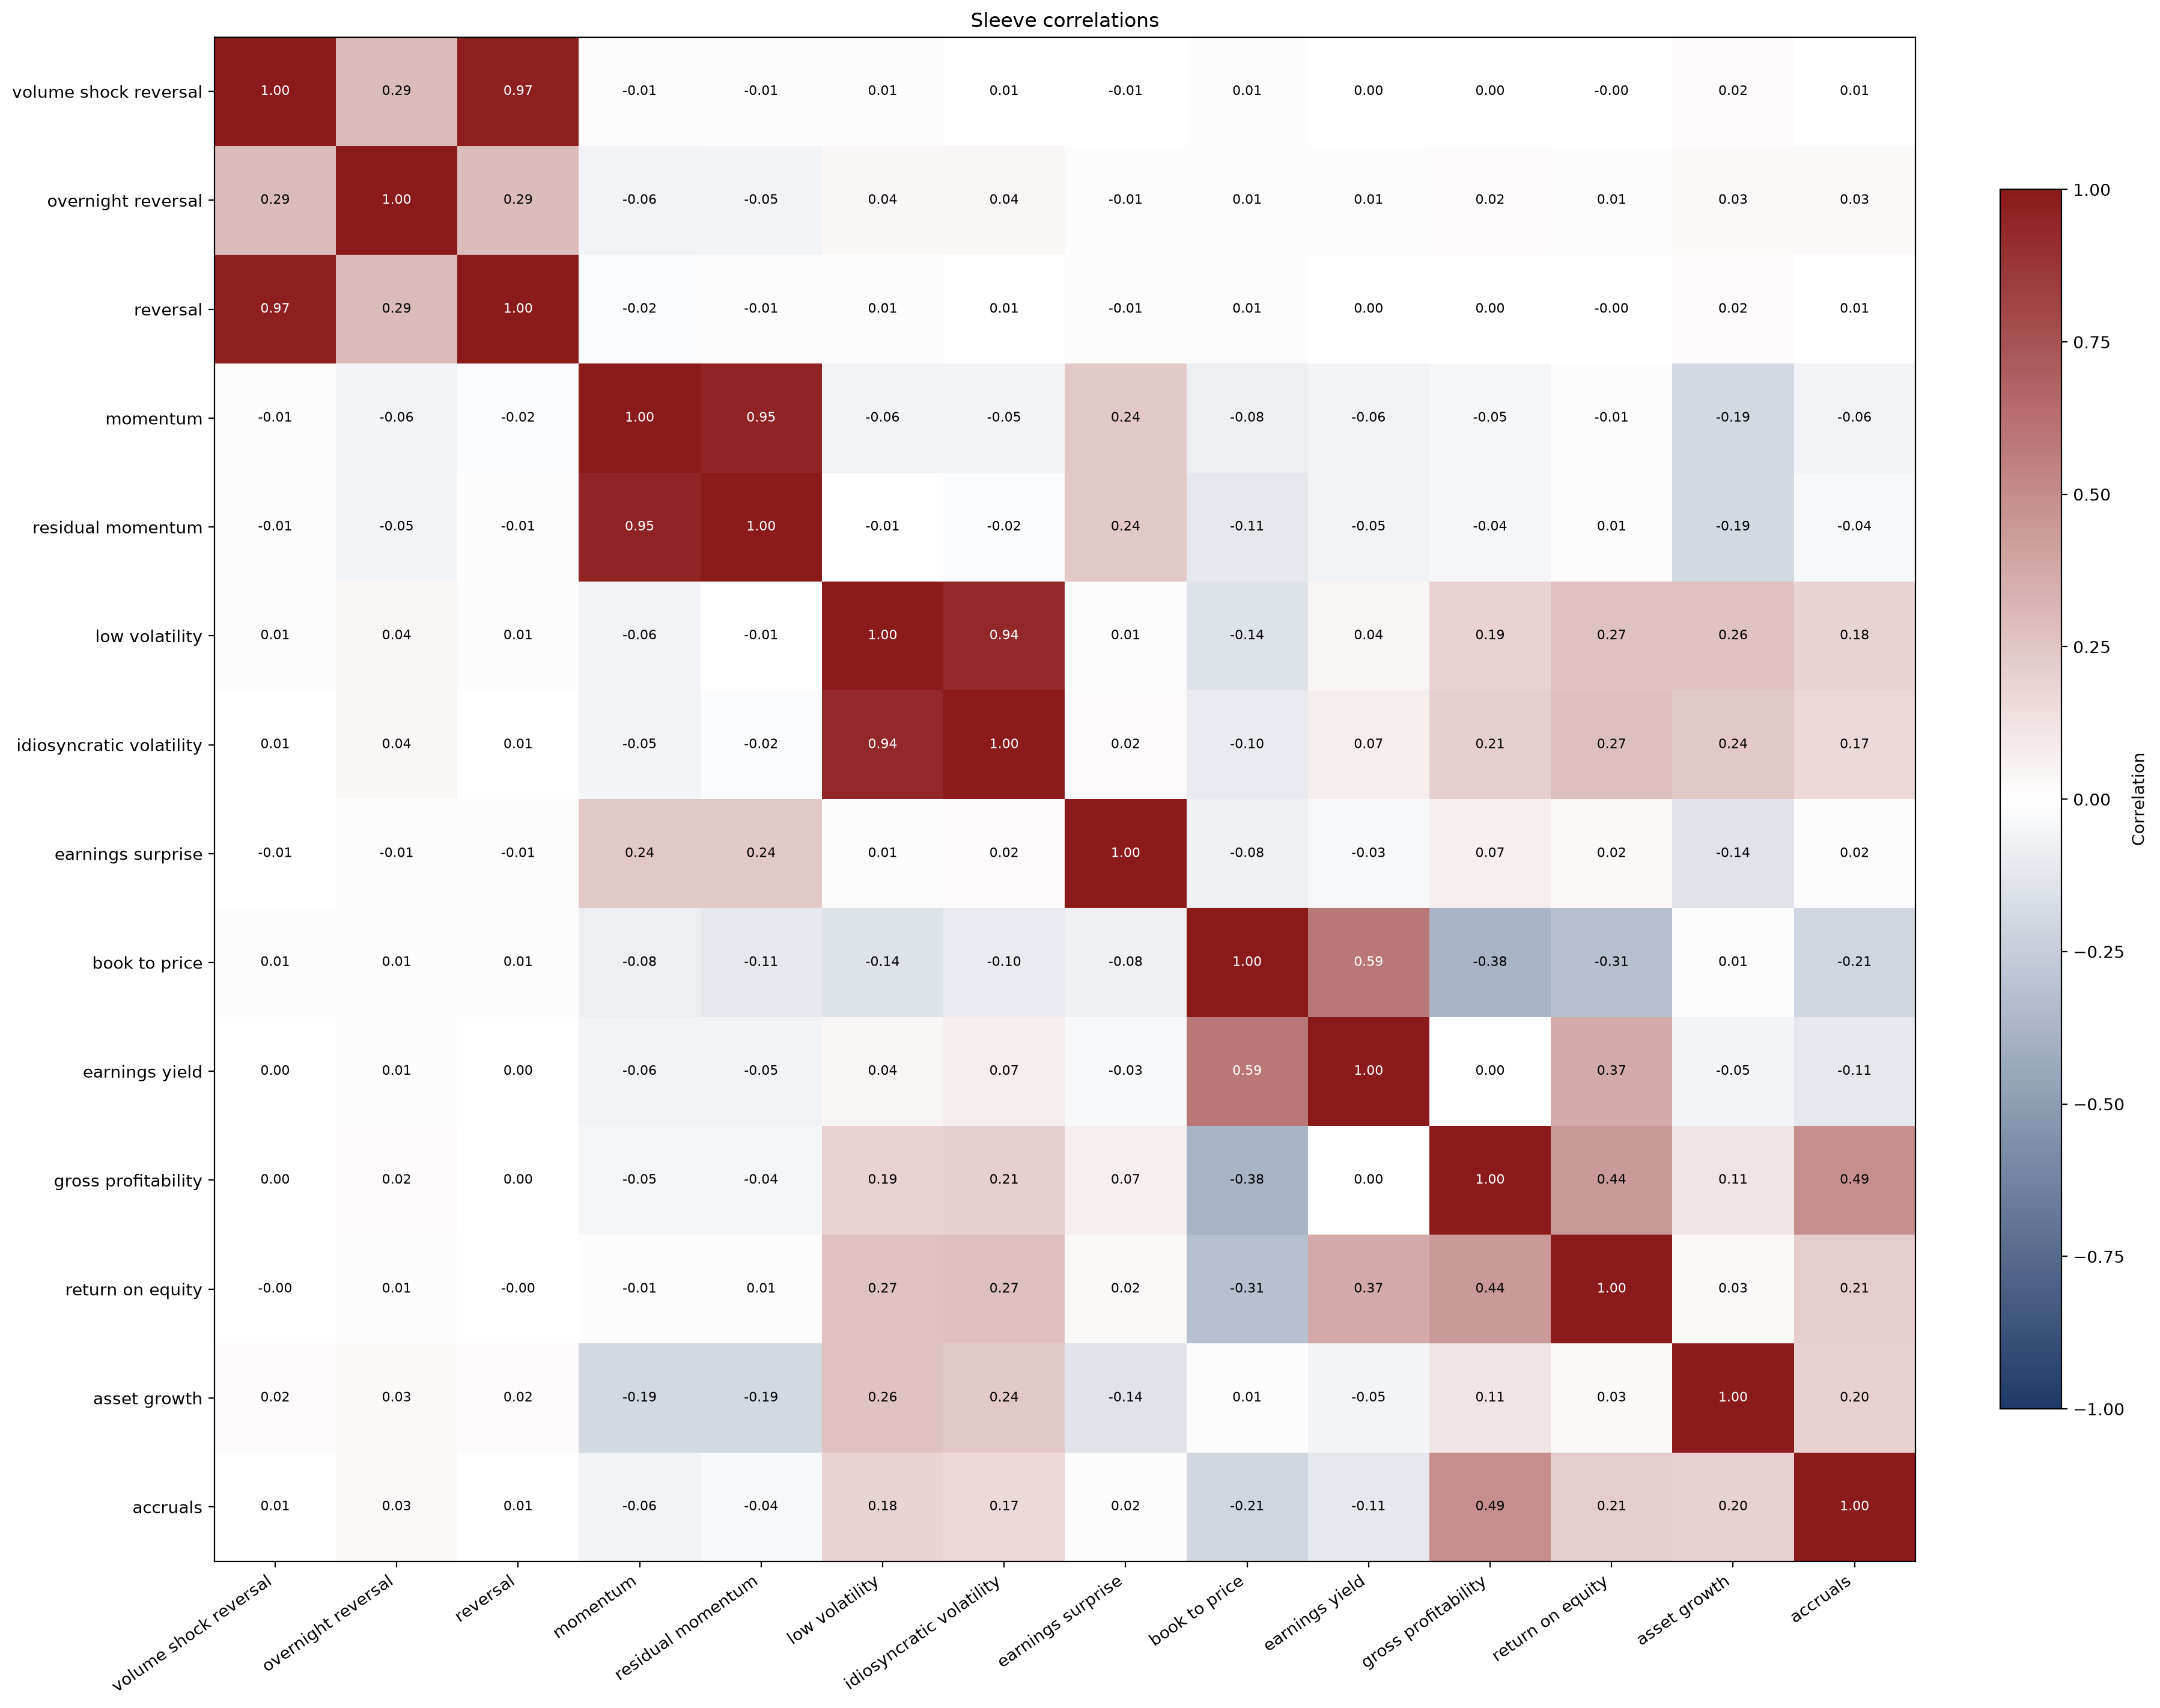
\includegraphics[width=0.84\textwidth]{sleeve_correlations.png}}{\fbox{\parbox[c][2.5cm][c]{0.7\linewidth}{\centering\small Missing figure: sleeve\_correlations.png}}}
\caption{Correlation structure of candidate alpha sleeves. Variants within a family are highly redundant, whereas the selected sleeves are comparatively weakly correlated.}
\label{fig:corr}
\end{figure}

\section{Portfolio Construction and Risk Controls}
\label{sec:portfolio}

The raw score is converted into positions using inverse-volatility scaling and a covariance model. A 252-day Ledoit--Wolf shrinkage covariance matrix is estimated over the names tradable at each refresh date and updated every 21 trading days. Shrinkage is used because covariance estimation becomes unstable when the cross-section is large relative to the available sample \citep{ledoitwolf2004}.

Each name's raw position is its score divided by its volatility (the square root of the corresponding diagonal element of $\Sigma$); the full covariance matrix enters through the volatility target. The position vector is multiplied by a scalar chosen to target 10\% annualized ex-ante volatility,
\begin{equation}
 \sigma_p = \sqrt{252\,w^\top \Sigma w}.
\end{equation}
In practice, the 1.5\% single-name limit binds before the 10\% volatility target can be reached. The delivered portfolio therefore realizes only about 3.34\% ex-ante volatility and 3.65\% ex-post annualized volatility. This is not a software failure; with approximately 100 names and a tight per-name cap, the maximum attainable idiosyncratic risk is arithmetically limited.

Dollar, beta, and sector neutrality are enforced jointly. Let $X_t$ contain an intercept, estimated market beta, and sector dummy exposures. The unconstrained position vector $\tilde w_t$ is projected onto the orthogonal complement of the exposure space,
\begin{equation}
 w_t^{(0)}=\left[I-X_t(X_t^\top X_t)^{-1}X_t^\top\right]\tilde w_t.
\end{equation}
The implementation evaluates this projection with a least-squares solve rather than by forming the inverse, because $X_t$ is routinely rank-deficient: a sector holding a single tradable name is collinear with the intercept, and a sector with no members on a given day contributes a column of zeros.

Because clipping to position and liquidity limits can reintroduce factor exposures while re-projection can violate caps, the algorithm iterates eight times through the sequence project, rescale to the volatility target, clip to the per-name and liquidity caps, and cap gross exposure. A final projection then restores exact neutrality, and a single uniform scale-down brings every hard limit back into force without disturbing it.

The principal portfolio constraints are summarized in Table~\ref{tab:params}.

\begin{table}[H]
\centering
\caption{Key strategy parameters.}
\label{tab:params}
\begin{tabular}{lll}
\toprule
Parameter & Value & Interpretation \\
\midrule
Reversal lookback & 2 days & Return horizon reverted by volume-shock sleeve \\
Overnight lookback & 5 days & Overnight gaps accumulated for reversal \\
Volume baseline & 63 days & Reference window for abnormal volume \\
Earnings decay & 60 days & Linear decay horizon for PEAD signal \\
PEAD blend weight & 10\% & Remaining 90\% split evenly across reversal sleeves \\
Beta lookback & 126 days & Rolling stock beta estimate \\
Covariance lookback & 252 days & Ledoit--Wolf covariance window \\
Covariance refresh & 21 days & Approximate monthly update \\
Volatility target & 10\% annualized & Pre-cap ex-ante target \\
Single-name cap & 1.5\% of NAV & Maximum absolute position \\
Gross exposure cap & 3.0$\times$ NAV & Sum of absolute portfolio weights \\
ADV participation cap & 1\% & Maximum position relative to dollar volume \\
Rebalance interval & 10 trading days & Target positions updated every tenth day \\
No-trade band & 0.6\% of NAV & Suppress small target changes \\
Minimum trade & \$200 & Avoid uneconomic small orders \\
\bottomrule
\end{tabular}
\end{table}

The realized portfolio is much less levered than the formal gross cap: gross exposure averages about 1.00$\times$ NAV, with approximately 50\% long and 50\% short. Realized beta to the equal-weight tradable universe is 0.009, and average net dollar exposure is $-0.007$ of NAV.

Those are averages, and the distinction matters. Neutrality holds exactly in the \emph{target} weights by construction, but the held book drifts between rebalance dates as prices move, so the constraints bind only on trading days. Median absolute net dollar exposure of the held book is \textbf{[TODO]}\% of NAV with a maximum of \textbf{[TODO]}\%, against the $-0.007$ sample mean. The near-zero averages are therefore evidence that the residual exposure is unbiased, not that the portfolio is neutral at every moment.

\section{Execution and Transaction-Cost Model}
\label{sec:execution}

Signals are formed using information through the close of day $t$ and are executed at the next open, eliminating same-close execution assumptions. The book is rebalanced every ten trading days, and positions drift between rebalance dates. Trading is therefore concentrated: the portfolio generates roughly 53 orders on each rebalance day and none in between. Averaged over all 2,516 days, including the warm-up year with no trading, this is 4.77 trades per day. The design brief set a target band of 5--50 trades per day. The delivered configuration sits marginally below that band on a calendar-day average and above it on each rebalance day, because concentrating turnover into every tenth day is what net-Sharpe optimization selected; the band is therefore reported rather than satisfied.

Transaction costs are applied to every trade. The model includes:
\begin{itemize}
  \item tiered commissions of \$0.0035 per share with a \$0.35 minimum per order and a 1\% cap on trade value;
  \item SEC Section 31 and FINRA trading-activity fees on sales;
  \item a 0.5\% annualized borrow rate on short market value;
  \item a calibrated half-spread of roughly 0.44 basis points for the large-cap universe; and
  \item square-root market impact of the form
  \begin{equation}
    \mathrm{impact}_{i,t}=c\,\sigma_{i,t}\sqrt{\frac{Q_{i,t}}{\mathrm{ADV}_{i,t}}}, \qquad c=0.10,
  \end{equation}
  where $Q_{i,t}$ is shares traded, $\mathrm{ADV}_{i,t}$ is here the trailing 63-day average daily volume in shares, and $\sigma_{i,t}$ is the trailing 63-day standard deviation of daily returns, lagged one day.
\end{itemize}

Daily-bar spread estimators were tested and rejected for this application. Corwin--Schultz \citep{corwinschultz2012} and Abdi--Ranaldo \citep{abdiranaldo2017} produced implausible estimates for highly liquid mega-cap equities because daily range volatility dominates sub-basis-point bid--ask spreads. The final implementation therefore uses a transparent ADV-calibrated spread function rather than a nominally more sophisticated estimator outside its useful regime.

\begin{table}[H]
\centering
\caption{Annualized transaction-cost attribution for the delivered configuration.}
\label{tab:costs}
\begin{tabular}{lrrl}
\toprule
Component & bps of NAV/year & Share & Primary scaling variable \\
\midrule
Borrow & 25.16 & 39.6\% & Short market value and holding time \\
Slippage & 20.50 & 32.3\% & Spread and square-root impact per trade \\
Commission & 14.00 & 22.0\% & Shares traded and order minimum \\
Regulatory fees & 3.86 & 6.1\% & Sale proceeds and shares sold \\
Financing & 0.00 & 0.0\% & Borrowed cash \\
\midrule
Total & 63.52 & 100\% & 2.50 bps per dollar traded \\
\bottomrule
\end{tabular}
\end{table}

\begin{figure}[H]
\centering
\IfFileExists{cost_attribution.png}{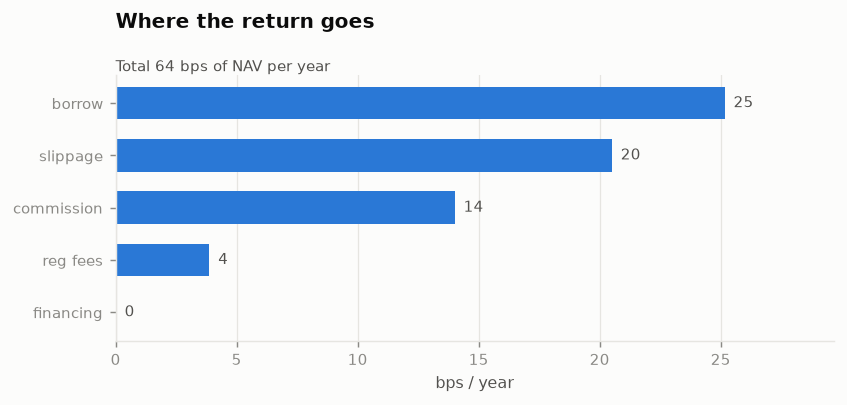
\includegraphics[width=0.76\textwidth]{cost_attribution.png}}{\fbox{\parbox[c][2.5cm][c]{0.7\linewidth}{\centering\small Missing figure: cost\_attribution.png}}}
\caption{Annual cost attribution. Borrow is the largest component, while slippage and commissions dominate the turnover-sensitive portion of the cost budget.}
\label{fig:costs}
\end{figure}

\section{Backtest and Validation Protocol}
\label{sec:validation}

The primary objective of the validation framework is to prevent research choices from being mislabeled as out-of-sample evidence. Several controls address data timing, parameter selection, non-normal returns, and multiple testing.

\subsection{Walk-forward evaluation}

The headline validation result uses thirteen consecutive six-month (126-day) out-of-sample folds. Each test window is preceded by an expanding training window that starts at the beginning of the sample with an initial length of 756 days. The ten-day holding period is embargoed from the end of the training sample so positions initiated in training cannot overlap test-period outcomes.

Three parameters are re-selected inside each training window---the earnings-sleeve weight, the rebalance interval, and the no-trade band---giving 27 candidate configurations per fold. The reversal lookback, the universe size, and the sleeve set are held fixed across all folds. Because each of those three was chosen by inspecting full-sample diagnostics, they are counted in the trial ledger but are not themselves validated out of sample, and the reported out-of-sample Sharpe is conditional on that structural choice. This is a substantive limitation of the design rather than a presentational one: a parameter fixed with full-sample knowledge transmits that knowledge into every fold.

\begin{figure}[H]
\centering
\IfFileExists{walk_forward_folds.png}{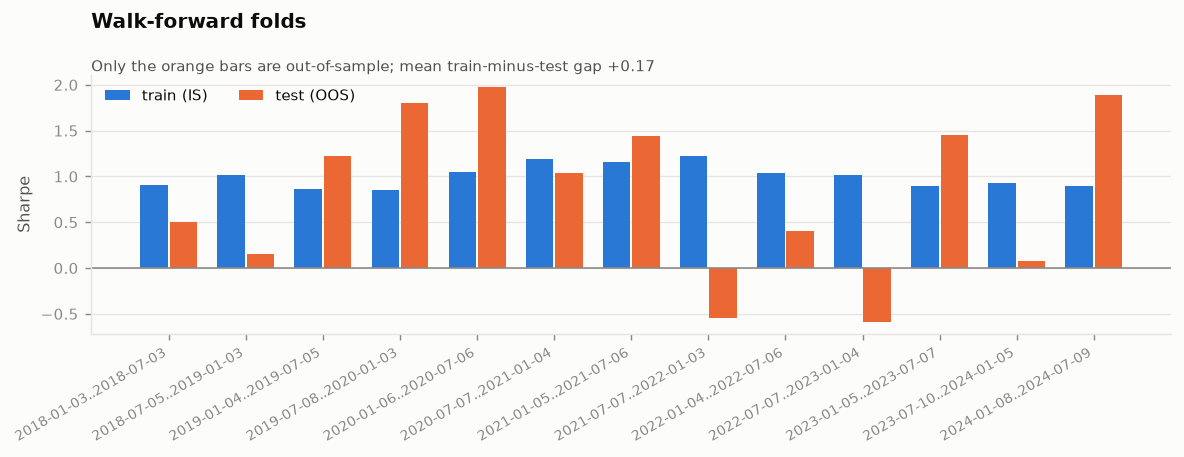
\includegraphics[width=0.86\textwidth]{walk_forward_folds.png}}{\fbox{\parbox[c][2.5cm][c]{0.7\linewidth}{\centering\small Missing figure: walk\_forward\_folds.png}}}
\caption{Training and test Sharpe ratios across the thirteen walk-forward folds. Eleven of thirteen test periods are positive, with an average train-minus-test gap of approximately 0.17 Sharpe units.}
\label{fig:walkforward}
\end{figure}

The final walk-forward out-of-sample Sharpe ratio is 0.901. A fixed-default portfolio evaluated on the same windows produces 0.951, indicating that per-fold parameter selection does not create the result and in fact carries a modest selection cost. Eleven of thirteen folds are profitable. The lower figure is nevertheless reported as the headline, because the fixed defaults were themselves chosen by examining full-sample results and 0.951 is therefore not a legitimately out-of-sample quantity; 0.901 is what a researcher obtains who must choose without seeing the test windows.

\subsection{Multiple testing and sampling uncertainty}

All research configurations examined are counted, including rejected experiments. The trial ledger contains 327 configurations; the final study adds the 28 runs of its own walk-forward grid (27 grid cells plus the base configuration), so the deflation is charged for 355 trials in total. The resulting Deflated Sharpe Ratio is 0.677, explicitly discounting the out-of-sample Sharpe for selection bias and non-normality following \citet{bailey2014}. The estimated probability of backtest overfitting is 0.216, computed by combinatorially symmetric cross-validation \citep{bailey2017} over the 28 walk-forward-grid configurations; it measures overfitting within that final grid, not across the full research history. The probabilistic Sharpe measure is 0.990.

Sampling uncertainty is evaluated using a 21-day block bootstrap, which preserves short-run dependence and volatility clustering better than independent daily resampling. The 95\% bootstrap interval for the out-of-sample Sharpe is $[0.23,1.59]$, with only 0.35\% of bootstrap draws below zero. That frequency and the probabilistic Sharpe measure of 0.990 both estimate the probability that true skill is positive, but they are not the same statistic---the first is a resampling frequency, the second a parametric adjustment for skewness and kurtosis---and the modest gap between them reflects that difference rather than an inconsistency. The interval is intentionally reported alongside the point estimate because ten years of daily data do not imply ten years of independent evidence.

\begin{figure}[H]
\centering
\begin{subfigure}{0.49\textwidth}
  \centering
  \IfFileExists{bootstrap_sharpe.png}{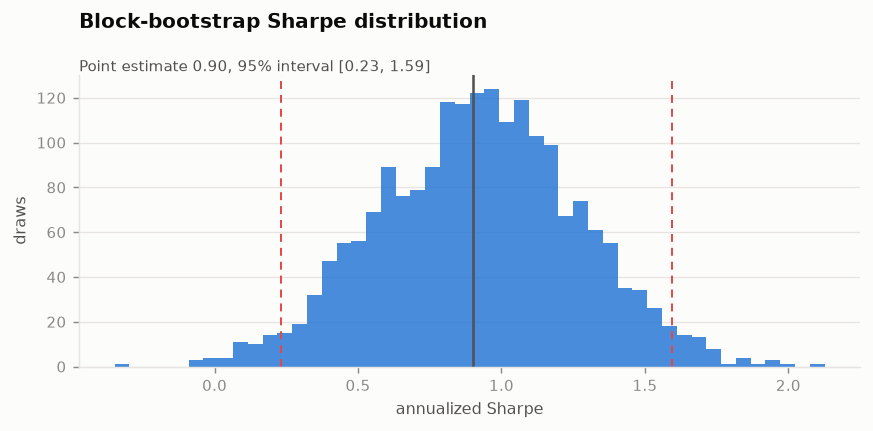
\includegraphics[width=\textwidth]{bootstrap_sharpe.png}}{\fbox{\parbox[c][2.5cm][c]{0.7\linewidth}{\centering\small Missing figure: bootstrap\_sharpe.png}}}
  \caption{Block-bootstrap distribution of Sharpe.}
\end{subfigure}\hfill
\begin{subfigure}{0.49\textwidth}
  \centering
  \IfFileExists{cost_sensitivity.png}{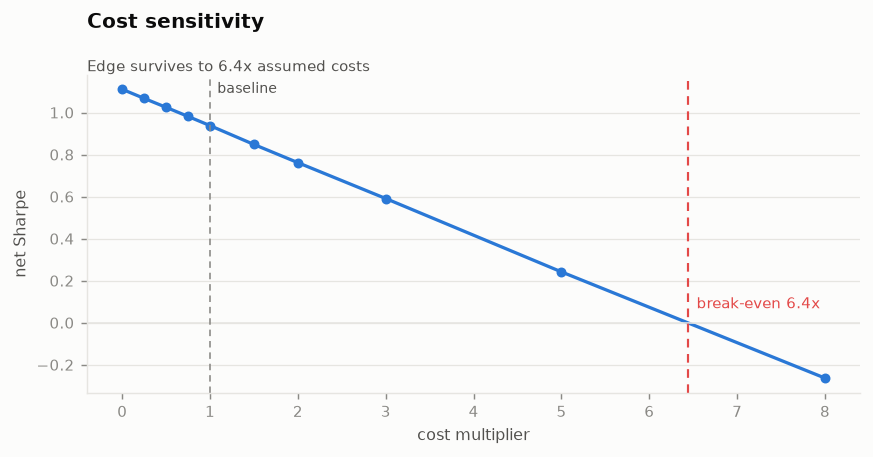
\includegraphics[width=\textwidth]{cost_sensitivity.png}}{\fbox{\parbox[c][2.5cm][c]{0.7\linewidth}{\centering\small Missing figure: cost\_sensitivity.png}}}
  \caption{Sharpe under proportional scaling of all modeled costs.}
\end{subfigure}
\caption{Uncertainty and cost-stress tests. The bootstrap quantifies sampling dispersion, while the cost sweep shows a break-even multiple of approximately 6.44 times the base-case cost model.}
\label{fig:validation}
\end{figure}

\subsection{Engine-level verification}

The backtesting engine is also checked independently of strategy performance. With the no-trade band disabled and full daily rebalancing, the engine's gross return matches an independent vectorized calculation to approximately $10^{-17}$. A causality test verifies that truncating future data does not change prior portfolio weights. Timing checks shift portfolio weights forward and backward by a day and confirm that performance changes materially, as it should if the engine is actually using the claimed next-open timing.

\begin{table}[H]
\centering
\caption{Primary validation diagnostics.}
\label{tab:validation}
\small
\begin{tabular}{p{0.29\textwidth}p{0.16\textwidth}p{0.47\textwidth}}
\toprule
Diagnostic & Result & Interpretation \\
\midrule
Walk-forward OOS Sharpe & 0.901 & Parameters selected from prior data only \\
Fixed-default OOS Sharpe & 0.951 & Same windows without per-fold reselection \\
Train minus test Sharpe & +0.168 & Estimated overfitting premium \\
Positive folds & 11/13 & Result not concentrated in one period \\
Probabilistic Sharpe & 0.990 & Probability true Sharpe exceeds zero under stated adjustment \\
Deflated Sharpe & 0.677 & Adjusted for 355 trials (327 ledger + 28 final grid) and non-normality \\
PBO & 0.216 & Probability of backtest overfitting within the 28-configuration final grid \\
Bootstrap 95\% CI & [0.23, 1.59] & Sampling uncertainty in OOS Sharpe \\
Minimum track record & 822 days & Reported threshold versus 1,638 OOS days available \\
Cost break-even & 6.44$\times$ & Full-sample multiple of modeled cost at which net Sharpe reaches zero, interpolated between the 5$\times$ and 8$\times$ sweep points \\
\bottomrule
\end{tabular}
\end{table}

\section{Results}
\label{sec:results}

Table~\ref{tab:performance} summarizes the delivered full-sample portfolio. Gross Sharpe is 1.111 and net Sharpe is 0.938 after all modeled trading and financing costs. The net annualized return is 3.41\% at 3.65\% annualized volatility. Maximum drawdown is 5.10\%, but the more informative statistic is duration: the worst drawdown lasts approximately 440 trading days from its prior peak to full recovery. The strategy therefore exhibits a relatively shallow but potentially difficult persistence of underperformance.

\begin{table}[H]
\centering
\caption{Full-sample portfolio performance, 2015--2024.}
\label{tab:performance}
\begin{tabular}{lrr}
\toprule
Metric & Gross & Net \\
\midrule
Sharpe ratio & 1.111 & 0.938 \\
Sortino ratio & 1.136 & 0.957 \\
Calmar ratio & 0.854 & 0.669 \\
Annualized return & 4.07\% & 3.41\% \\
Annualized volatility & 3.65\% & 3.65\% \\
Maximum drawdown & $-4.77$\% & $-5.10$\% \\
Drawdown duration & 417 days & 440 days \\
Hit rate & 52.3\% & 51.6\% \\
Win/loss ratio & 1.120 & 1.117 \\
95\% historical VaR & 0.33\% & 0.33\% \\
95\% CVaR & 0.48\% & 0.48\% \\
Skewness & 0.562 & 0.555 \\
Excess kurtosis & 7.14 & 7.20 \\
\bottomrule
\end{tabular}
\end{table}

All full-sample statistics in Table~\ref{tab:performance} are averaged over all 2,516 days, including the 260-day warm-up in which the book holds no positions and earns zero. Measured over the live period alone, annualized return, turnover, and costs are roughly 11\% higher and volatility and Sharpe roughly 6\% higher; the walk-forward results, which begin in 2018, are unaffected.

The return distribution is positively skewed but strongly leptokurtic, so Gaussian approximations understate tail thickness. The positive sign deserves comment because it runs against the usual characterization of a liquidity-providing strategy, which is expected to collect small premia routinely and suffer occasional large losses. No mechanism for the observed sign is established here; the leptokurtosis is in any case the feature that matters for the Deflated Sharpe adjustment of Section~\ref{sec:validation}. Annualized turnover is 25.4 times NAV on a one-way basis. The average order is about 0.04\% of the name's daily share volume, and the liquidity constraint, which caps each \emph{position} at 1\% of ADV, never binds at the tested capital scale.

\begin{figure}[H]
\centering
\IfFileExists{equity_drawdown.png}{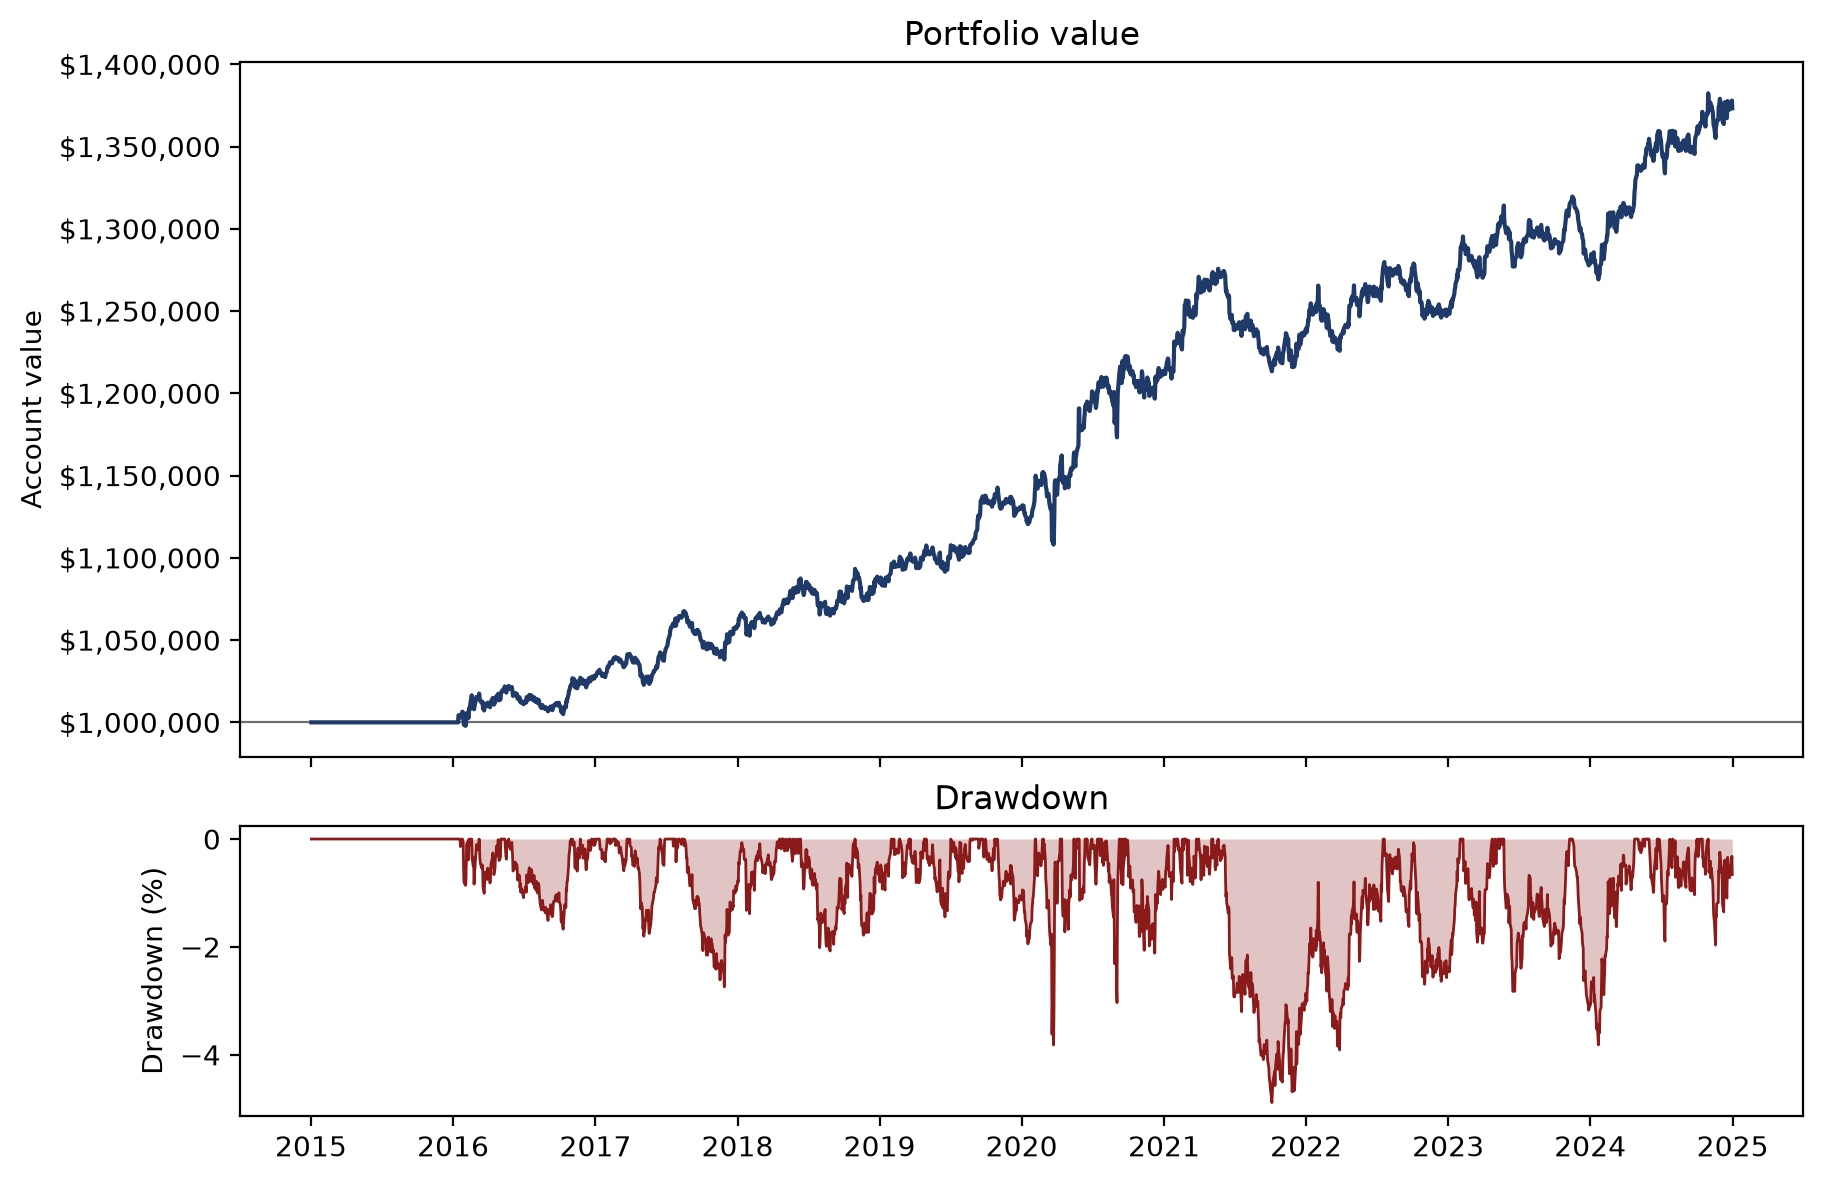
\includegraphics[width=0.88\textwidth]{equity_drawdown.png}}{\fbox{\parbox[c][2.5cm][c]{0.7\linewidth}{\centering\small Missing figure: equity\_drawdown.png}}}
\caption{Net equity curve and drawdown for a \$1 million capital run. This capacity illustration ends at approximately \$1.41 million after ten years. The drawdown panel emphasizes the long recovery periods hidden by the cumulative equity curve.}
\label{fig:equity}
\end{figure}

Figure~\ref{fig:equity} uses a \$1 million capital run rather than the \$10 million base parameterization because the project explicitly evaluates capital-size dependence. At \$1 million, the net Sharpe is approximately 0.954, slightly above the 0.938 value at \$10 million because market impact is smaller. At \$100,000 the Sharpe falls to approximately 0.89 as fixed commissions consume more return. At \$10,000, the strategy is infeasible: the 1.5\% cap limits every position to \$150, below the \$200 minimum-trade rule, so no order is ever placed. (The default capacity sweep spans \$1 million to \$1 billion; the \$100,000 and \$10,000 cases come from a supplementary run of the same pipeline.) Capacity is therefore two-sided: fixed order costs dominate at small NAV while impact dominates as NAV grows.

\begin{figure}[H]
\centering
\IfFileExists{rolling_sharpe.png}{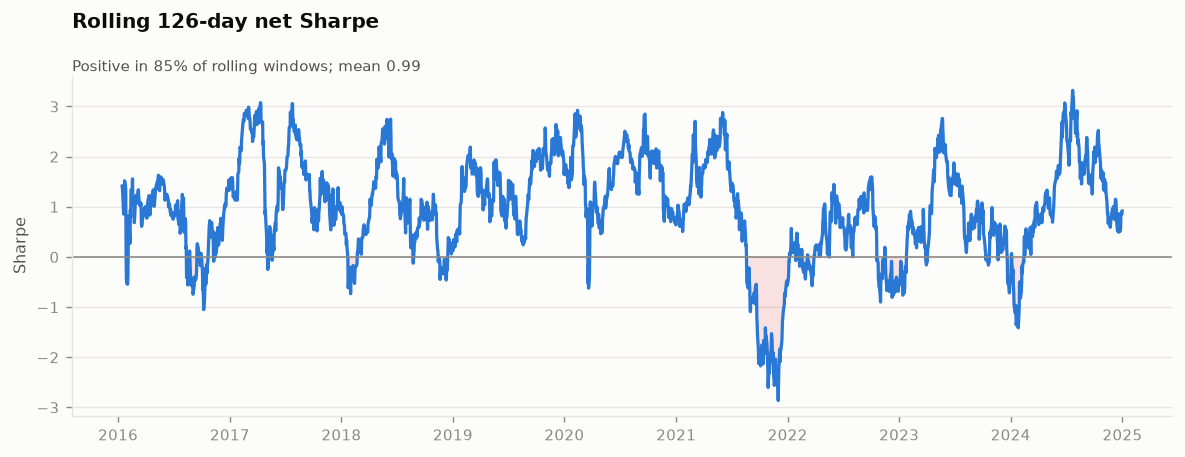
\includegraphics[width=0.86\textwidth]{rolling_sharpe.png}}{\fbox{\parbox[c][2.5cm][c]{0.7\linewidth}{\centering\small Missing figure: rolling\_sharpe.png}}}
\caption{Rolling 126-trading-day net Sharpe. Approximately two thirds of windows are positive, but the strategy experiences sustained weak regimes.}
\label{fig:rolling}
\end{figure}

The rolling evidence reinforces the importance of regime variation. The full-sample Sharpe is not generated by a uniformly smooth return process. Extended weak intervals remain even after combining signals, which is consistent with the 440-day maximum drawdown duration.

\section{Diagnostic Decomposition}
\label{sec:diagnostics}

A central contribution of the project is the use of the Fundamental Law of Active Management as a diagnostic rather than a decorative identity. In the project's notation,
\begin{equation}
 \IR = \TC\,\IC\,\sqrt{\BR},
 \label{eq:fundlaw}
\end{equation}
where $\IC$ is forecasting skill, $\BR$ is effective breadth, and $\TC$ summarizes how much of the ideal alpha survives portfolio construction and implementation \citep{grinold1989,grinoldkahn2000}. The transfer coefficient in the form used here---the cross-sectional correlation between the unconstrained and the delivered portfolio---follows \citet{clarke2002}.

\begin{table}[H]
\centering
\caption{Fundamental-Law diagnostics.}
\label{tab:fundlaw}
\small
\begin{tabular}{p{0.30\textwidth}p{0.16\textwidth}p{0.46\textwidth}}
\toprule
Term & Measured value & Interpretation \\
\midrule
Information coefficient & 0.0113 & Daily rank correlation; $t=2.55$ \\
IC hit rate & 50.8\% & Fraction of days with positive IC \\
Naive breadth & 25,193 & 100 names $\times$ 252 days under independence \\
Independent directions & 24.6 & Effective cross-sectional dimensions among 100 names \\
Signal autocorrelation & 0.652 & Persistence reduces independent decisions over time \\
Effective breadth & 1,309 & About 19$\times$ below the naive count \\
Constraint transfer coefficient & 0.631 & Correlation of ideal (pre-constraint) and post-constraint target weights \\
Cost transfer coefficient & 0.844 & Net Sharpe divided by gross Sharpe (0.938/1.111) \\
\bottomrule
\end{tabular}
\end{table}

\begin{figure}[H]
\centering
\IfFileExists{effective_breadth.png}{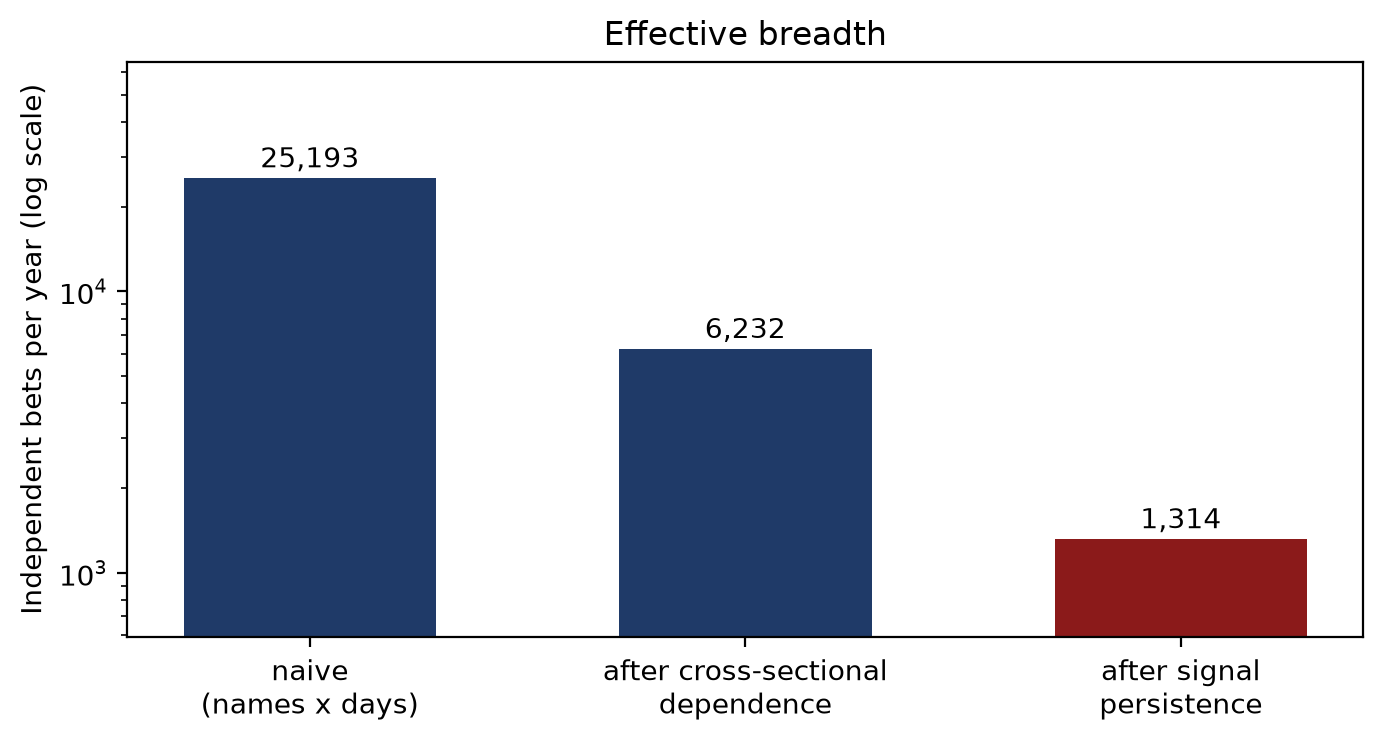
\includegraphics[width=0.72\textwidth]{effective_breadth.png}}{\fbox{\parbox[c][2.5cm][c]{0.7\linewidth}{\centering\small Missing figure: effective\_breadth.png}}}
\caption{Reduction from naive breadth to effective breadth after accounting for cross-sectional dependence and signal persistence.}
\label{fig:breadth}
\end{figure}

The diagnostic explains several otherwise counterintuitive findings. First, a strong standalone information coefficient is not sufficient if the signal hardly changes. Several value and quality ratios constructed from SEC data have autocorrelations above 0.997 and therefore contribute almost no effective breadth. By contrast, the earnings-surprise signal has an event clock and staggered fiscal timing, making it useful despite only modest standalone skill.

Second, loosening portfolio constraints is not necessarily beneficial. In experiments on the earlier two-sleeve book (before the earnings sleeve was added), changes that increased the constraint transfer coefficient from 0.63 to 0.84 by relaxing position caps, dropping sector neutrality, or moving toward mean--variance weights reduced net Sharpe from roughly 0.78 to 0.39; gross Sharpe also fell. The constraints therefore behave like regularization against a noisy alpha estimate, consistent with the broader result that apparently ``wrong'' constraints can improve out-of-sample portfolio risk \citep{jagannathanma2003}.

Third, the largest improvement in the research process came from combining weakly correlated forecasts rather than searching for a single dominant predictor. It is worth being explicit about which term in \eqref{eq:fundlaw} this affects, since the two are easily conflated. Breadth as measured here is a property of the \emph{opportunity set}: the number of independent return directions in the cross-section multiplied by the number of independent rebalancing decisions per year. Blending sleeves changes neither. For $S$ standardized forecasts of equal individual skill $c$ and average pairwise correlation $\bar{\rho}$, the equal-weighted composite satisfies
\begin{equation}
\IC_{\text{blend}} = c\,\sqrt{\frac{S}{1 + (S-1)\bar{\rho}}},
\label{eq:blendic}
\end{equation}
so diversification across signals raises $\IC$ at fixed $\BR$. Because $\IR$ is linear in $\IC$ and proportional to $\sqrt{\BR}$, a factor of $\sqrt{S}$ obtained from uncorrelated sleeves is numerically indistinguishable from an $S$-fold increase in breadth, which is why the two are often described interchangeably. The distinction matters here because the two levers were available to different degrees: additional sleeves could be constructed, whereas breadth was fixed by the universe and by the persistence of the signal. The rise in gross Sharpe from 0.68 to 0.91 on combining volume-shock and overnight reversal is therefore an $\IC$ effect, and the 19-fold breadth reduction in Table~\ref{tab:fundlaw} is the constraint against which it was spent. Section~\ref{sec:robustness} provides the empirical separation: six sleeves with near-zero correlation to the price signals contributed nothing, because independence in the forecast cannot substitute for breadth in the opportunity set.

\section{Robustness, Extensions, and Negative Results}
\label{sec:robustness}

Several substantial research directions were measured and then rejected. Including negative results is important because the reported strategy emerged from a search process whose unsuccessful branches still contribute to multiple-testing risk.

\subsection{Liquidity spectrum}

The project tests the idea that reversal should be stronger in less-liquid stocks across 1,448 S\&P 1500 names. The measured difference in information coefficient between the least and most liquid deciles is only 0.0001 with a $t$-statistic of 0.02, while estimated spreads rise sharply as liquidity falls. The most liquid decile therefore provides the best signal per basis point of spread paid, and the full strategy's net Sharpe peaks at roughly 100 names before declining at 200, 400, and 800.

\begin{figure}[H]
\centering
\IfFileExists{liquidity_deciles.png}{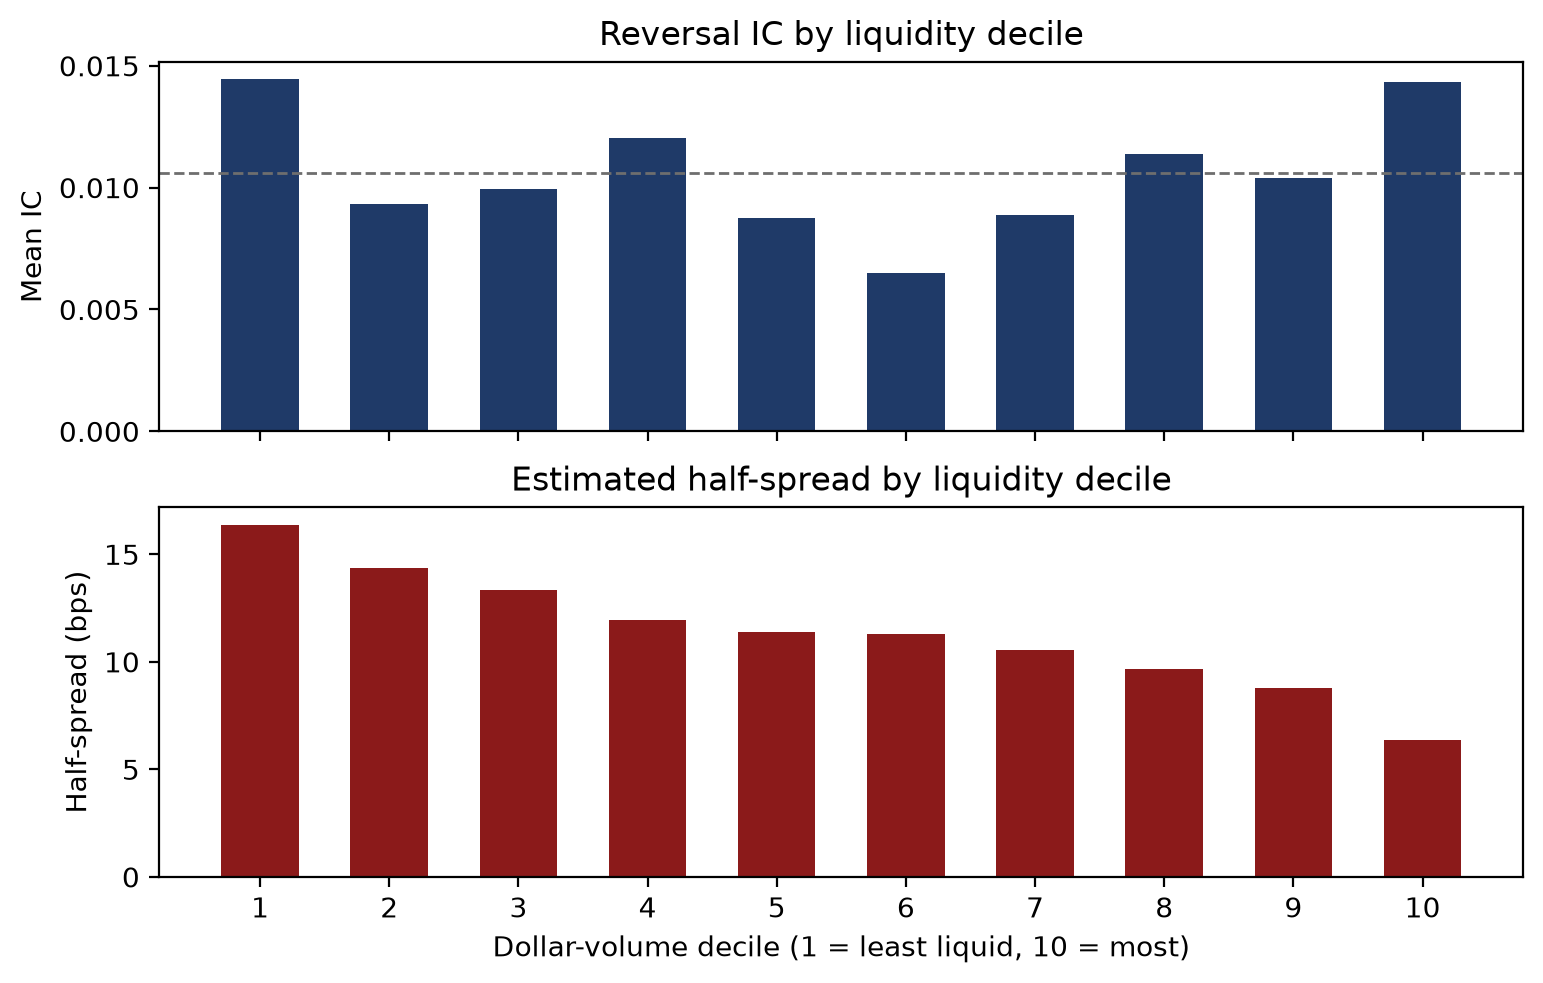
\includegraphics[width=0.78\textwidth]{liquidity_deciles.png}}{\fbox{\parbox[c][2.5cm][c]{0.7\linewidth}{\centering\small Missing figure: liquidity\_deciles.png}}}
\caption{Information coefficient and estimated spread by dollar-volume decile in the broader liquidity study. Signal strength is essentially flat while trading costs rise materially in less-liquid names.}
\label{fig:liquidity}
\end{figure}

\subsection{Fundamental and insider extensions}

Six value and quality sleeves built from point-in-time SEC fundamentals are nearly uncorrelated with the price signals but fail to improve the portfolio because they change too slowly. A second research round evaluates SEC Form 4 insider activity and additional earnings cuts. Insider net buying has a significantly negative measured IC ($-0.0133$, $t=-3.50$), but the sign is not reversed for trading because doing so would amount to sample-driven curve fitting without a supporting mechanism. Revenue surprise produces an information coefficient of 0.0175 ($t=3.05$), the highest of any sleeve measured in the project, and is nonetheless rejected. Its cross-sectional score correlation with the existing earnings sleeve is 0.46, which by \eqref{eq:blendic} retains only about 41\% of the diversification benefit available at zero correlation; the decisive evidence, however, is direct. Substituting it for the earnings sleeve yields an out-of-sample net Sharpe of 0.806 and adding it alongside yields 0.791, against 0.864 for the delivered three-sleeve configuration. The rejection therefore rests on measured performance rather than on an undisclosed correlation threshold.

\subsection{Intraday reversal and passive execution}

Hourly reversal is statistically interesting: on 309,573 hourly bars it produces an IC of 0.0095 with a $t$-statistic of 2.9 and nearly zero autocorrelation, implying about 26,059 effective bets per year. The problem is execution. The research estimates that commission plus regulatory fees alone are approximately 0.700 basis points per dollar traded, while the maximum half-spread available to a perfectly passive order is only about 0.440 basis points. Even an unrealistically perfect passive execution process therefore cannot make turnover free. The intraday extension is rejected before a complex fill simulation is built.

\subsection{Regime conditioning and the no-trade band}

Cross-sectional dispersion appears to condition forecast IC monotonically, but scaling exposure with the regime fails a control test: a constant multiplier at the same average portfolio size achieves a Sharpe of 0.907 compared with 0.878 for the regime-varying rule. The improvement initially attributed to timing is instead explained by lower turnover. That finding leads to the true implementation lever---the no-trade band. Re-optimizing the band produces an interior optimum: net Sharpe rises from 0.845 with no band to 0.975 at a 1.0\% band, then drops sharply to 0.857 at 1.3\%. Bands above the 1.5\% single-name cap mechanically shut down trading, because no position can be opened by a trade larger than the cap. The delivered configuration uses 0.6\% rather than the 1.0\% peak, keeping a margin from that cliff, and the band is re-selected per fold in the walk-forward.

\begin{figure}[H]
\centering
\IfFileExists{pead_weight_sweep.png}{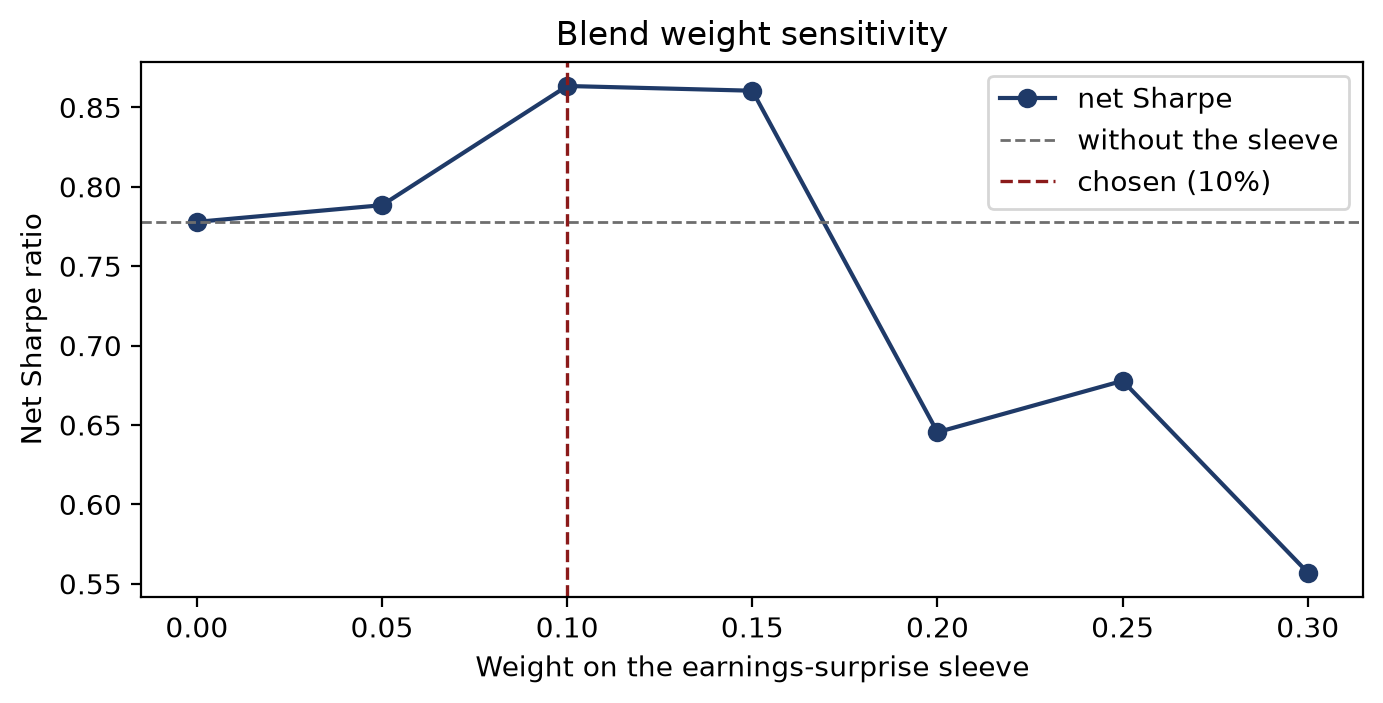
\includegraphics[width=0.72\textwidth]{pead_weight_sweep.png}}{\fbox{\parbox[c][2.5cm][c]{0.7\linewidth}{\centering\small Missing figure: pead\_weight\_sweep.png}}}
\caption{Sensitivity to the earnings-sleeve weight. The chosen 10\% allocation is the best cell of the sweep, with lower net Sharpe on either side, so the weight is re-selected within each walk-forward training window rather than fixed in advance.}
\label{fig:peadweight}
\end{figure}

\section{Limitations}
\label{sec:limitations}

The backtest includes more realism than a simple signal study, but several limitations bias the reported performance upward or widen the uncertainty around it.

\begin{enumerate}
  \item \textbf{Survivorship bias.} Historical trading is simulated using a universe seeded from current S\&P 500 membership, and yfinance does not provide a delisting-inclusive historical constituent panel. Failed or delisted firms are therefore missing. For a reversal strategy, this is especially consequential because some extreme losers do not recover. The result should be interpreted as an upper bound until point-in-time membership and delisting returns are incorporated.

  \item \textbf{Trading costs are modeled rather than observed.} Bid--ask spread and impact parameters are calibrated rather than estimated from quote-level data or live fills. Hard-to-borrow rates are modeled with a uniform 0.5\% annual borrow assumption, which may understate the cost of shorting recent winners. The 6.44$\times$ cost break-even result is therefore more informative than the precision of the 63.52 bps base case.

  \item \textbf{Fill uncertainty is absent.} Intended trades are assumed to execute fully at the modeled next-open price plus slippage. Real orders may be partially filled or experience additional gap and queue risk.

  \item \textbf{Sector classifications are not historical.} Current GICS labels are applied backward through time, so sector-neutrality constraints are not perfectly point-in-time.

  \item \textbf{Ten years remains one market sample.} The sample spans several distinct regimes, but it is not long enough to eliminate uncertainty about structural change. The broad bootstrap interval demonstrates that uncertainty directly.

  \item \textbf{Research search remains a source of optimism.} The trial ledger, Deflated Sharpe Ratio, PBO, and walk-forward design reduce but cannot eliminate the consequences of iterative human research decisions.
\end{enumerate}

These limitations are important when interpreting the 0.90 out-of-sample Sharpe. The result is evidence of a potentially persistent cross-sectional effect under the modeled conditions, not evidence that the same Sharpe would be achieved live.

\section{Reproducibility}
\label{sec:reproducibility}

The full study---baseline backtest, Fundamental-Law diagnostic, walk-forward, sensitivity grid, Deflated Sharpe, PBO, bootstrap, cost sweep, and capacity sweep---runs from a single command, \texttt{uv run quant-capstone run}, which writes a results report and figures. All defaults live in one configuration module, every sweep is recorded in the trial ledger, and the test suite covers signal construction, neutralization, cost accounting, and causality. The engine cross-checks of Section~\ref{sec:validation} are available as \texttt{uv run quant-capstone crosscheck}.

Exact numerical reproduction additionally requires the same data snapshot. Prices, the S\&P 500 constituent list, and SEC filings are downloaded at run time and cached locally; a later download picks up a different current constituent list and revised price adjustments, so headline statistics shift even though the code is unchanged. The figures in this report come from a single cached snapshot, and archiving that snapshot alongside the code is the remaining step needed for exact replication.

\section{Conclusion}

This project develops a market-neutral U.S. equity strategy that combines short-horizon reversal, overnight reversal, and an event-driven earnings signal within a realistic portfolio and execution framework. The final result is economically modest but statistically nontrivial: full-sample net Sharpe is 0.938, walk-forward out-of-sample Sharpe is 0.901, and the maximum drawdown is approximately 5.1\%. These returns survive a full modeled cost budget of roughly 64 basis points per year and remain positive under substantial cost inflation.

The most important lessons are methodological. First, combining genuinely different signals raises composite forecasting skill more reliably than refining a single predictor. Second, effective breadth---after correcting for cross-sectional dependence and signal persistence---is the binding resource. Third, portfolio constraints can improve rather than degrade realized performance by regularizing noisy forecasts. Fourth, realistic transaction costs change which research directions are worth pursuing: intraday breadth is attractive statistically but uneconomic under the tested fee structure. Finally, strong validation infrastructure matters as much as signal design. Causality checks, an embargoed walk-forward procedure, an explicit trial ledger, block-bootstrap uncertainty, and engine cross-checks all prevented plausible but incorrect conclusions from surviving into the final result.

The strategy should therefore be viewed as a disciplined empirical demonstration of quantitative research practice rather than a claim of immediately deployable alpha. The next substantive improvement is not another parameter sweep; it is better data. A point-in-time, delisting-inclusive universe and quote-level execution data would directly address the two largest remaining sources of optimism and allow the economic result to be evaluated on a materially stronger foundation.

\begin{thebibliography}{99}

\bibitem[Abdi and Ranaldo(2017)]{abdiranaldo2017}
Abdi, F. and Ranaldo, A. (2017).
A simple estimation of bid--ask spreads from daily close, high, and low prices.
\textit{The Review of Financial Studies}, 30(12), 4437--4480.

\bibitem[Bailey and L\'opez de Prado(2014)]{bailey2014}
Bailey, D. H. and L\'opez de Prado, M. (2014).
The Deflated Sharpe Ratio: Correcting for selection bias, backtest overfitting, and non-normality.
\textit{The Journal of Portfolio Management}, 40(5), 94--107.

\bibitem[Bailey et al.(2017)]{bailey2017}
Bailey, D. H., Borwein, J. M., L\'opez de Prado, M., and Zhu, Q. J. (2017).
The probability of backtest overfitting.
\textit{The Journal of Computational Finance}, 20(4), 39--69.

\bibitem[Bernard and Thomas(1989)]{bernard1989}
Bernard, V. L. and Thomas, J. K. (1989).
Post-earnings-announcement drift: Delayed price response or risk premium?
\textit{Journal of Accounting Research}, 27, 1--36.

\bibitem[Bernard and Thomas(1990)]{bernard1990}
Bernard, V. L. and Thomas, J. K. (1990).
Evidence that stock prices do not fully reflect the implications of current earnings for future earnings.
\textit{Journal of Accounting and Economics}, 13(4), 305--340.

\bibitem[Campbell et al.(1993)]{cgw1993}
Campbell, J. Y., Grossman, S. J., and Wang, J. (1993).
Trading volume and serial correlation in stock returns.
\textit{The Quarterly Journal of Economics}, 108(4), 905--939.

\bibitem[Clarke et al.(2002)]{clarke2002}
Clarke, R., de Silva, H., and Thorley, S. (2002).
Portfolio constraints and the fundamental law of active management.
\textit{Financial Analysts Journal}, 58(5), 48--66.

\bibitem[Corwin and Schultz(2012)]{corwinschultz2012}
Corwin, S. A. and Schultz, P. (2012).
A simple way to estimate bid--ask spreads from daily high and low prices.
\textit{The Journal of Finance}, 67(2), 719--760.

\bibitem[Grinold(1989)]{grinold1989}
Grinold, R. C. (1989).
The fundamental law of active management.
\textit{Journal of Portfolio Management}, 15(3), 30--37.

\bibitem[Grinold and Kahn(2000)]{grinoldkahn2000}
Grinold, R. C. and Kahn, R. N. (2000).
\textit{Active Portfolio Management: A Quantitative Approach for Providing Superior Returns and Controlling Risk}, 2nd ed.
McGraw--Hill, New York.

\bibitem[Jagannathan and Ma(2003)]{jagannathanma2003}
Jagannathan, R. and Ma, T. (2003).
Risk reduction in large portfolios: Why imposing the wrong constraints helps.
\textit{The Journal of Finance}, 58(4), 1651--1683.

\bibitem[Jegadeesh(1990)]{jegadeesh1990}
Jegadeesh, N. (1990).
Evidence of predictable behavior of security returns.
\textit{The Journal of Finance}, 45(3), 881--898.

\bibitem[Ledoit and Wolf(2004)]{ledoitwolf2004}
Ledoit, O. and Wolf, M. (2004).
A well-conditioned estimator for large-dimensional covariance matrices.
\textit{Journal of Multivariate Analysis}, 88(2), 365--411.

\bibitem[Lehmann(1990)]{lehmann1990}
Lehmann, B. N. (1990).
Fads, martingales, and market efficiency.
\textit{The Quarterly Journal of Economics}, 105(1), 1--28.

\bibitem[Lo and MacKinlay(1990)]{lomackinlay1990}
Lo, A. W. and MacKinlay, A. C. (1990).
When are contrarian profits due to stock market overreaction?
\textit{The Review of Financial Studies}, 3(2), 175--205.

\bibitem[Lou et al.(2019)]{lps2019}
Lou, D., Polk, C., and Skouras, S. (2019).
A tug of war: Overnight versus intraday expected returns.
\textit{Journal of Financial Economics}, 134(1), 192--213.

\bibitem[Bates and Granger(1969)]{batesgranger1969}
Bates, J. M. and Granger, C. W. J. (1969).
The combination of forecasts.
\textit{Operational Research Quarterly}, 20(4), 451--468.

\end{thebibliography}

\end{document}